\documentclass[../../main]{subfiles}
\begin{document}
    \section{Model Construction}
    ODE models in systems biology are best built from a visual representation of the network, otherwise it
    is easy to get get confused and make mistakes. The networks should be as tidy as possible. There is no use
    building a messy network with wires crossing wires everywhere because that detracts from the
    purpose of having a network: to guide your thinking about how the network is going to behave.

    Biochemical networks are often drawn in a cartoon format at the end of a mechanistic biology paper. These are often
    ambiguous and should be avoided. Instead, a good approach is to draw a wiring diagram (Figure \ref{fig:model_construction:wiring_diagram})
    on paper to get a network that seems reasonable and then use \href{http://www.celldesigner.org/}{CellDesigner} to make the representation
    more formal.

    \note{The arrows in these networks define the general relationship between model components,
    but not the exact mathematical relationship. For instance, an arrow between A and B might represent a
    mass action relationship or some other kind of rate law (i.e. Michaelis-Menten)}.

    \remember{A neat and tidy network is not just for aesthetics but will help you think about your network. }

    \begin{Task}[label=ToyWiringDiagram]{Toy Wiring Diagram}
        Draw a wiring diagram of a toy (made up) network. You will later simulate this network so make it interesting
        but don't over complicate it. You should include at least one Michaelis-Menten and one Competitive Inhibition
        reaction.
    \end{Task}

    \begin{figure}[t]
        \centering
        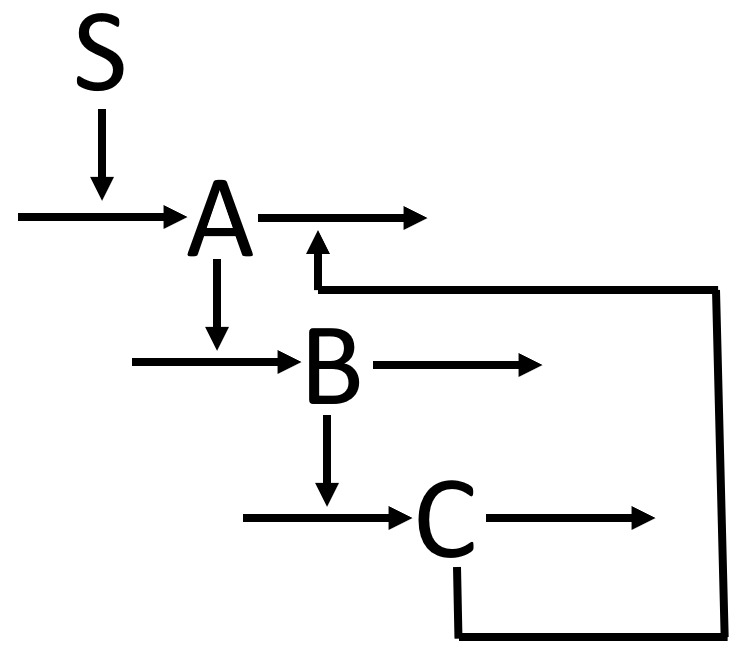
\includegraphics[width=0.5\linewidth]{ODEModels/ModelConstruction/assets/wiring_diagram.png}
        \caption[wiring diagram]{Example wiring diagram of a network where A is produced in response to stimulus S.
        Then a signal cascade begins, starting with A, flowing through B to C. C causes the degradation of A and
        therefore completes a negative feedback loop.}
        \label{fig:model_construction:wiring_diagram}
    \end{figure}


    \begin{Task}[label=CellDesigner]{Cell Designer}
        Draw the same network you drew for the wiring exercise using CellDesigner.
    \end{Task}

    \subsection{Antimony}
    Antimony is the name of a piece of software that has defined its own language for creating SBML models.
    The idea is that you build the model in this human-friendly format and then use the conversion tools
    provided for converting the antimony string into a simulatable model. The docs for antimony can be
    found \href{https://tellurium.readthedocs.io/en/latest/antimony.html}{here} and \href{http://tellurium.analogmachine.org/antimony-tutorial/}{here}.

    \begin{Task}[label=AntimonyString]{Build an Antimony String}
        Build an antimony version of your model using the documentation to help you.
        Assign your antimony to a variable inside {model_strings.py~} so that you can import the
        string inside the \bash{control_script.py}.
    \end{Task}

    It is not always obvious how to use Antimony and the docs are not always helpful
    for every question you might have. However, there is an alternative option. The tellurium package
    has fairly comprehensive conversion facilities that can directly convert SBML to antimony. This means
    that it is possible to build a SBML model using whichever tool you like and then convert it into an
    antimony string. Therefore, if you cannot figure out how to implement a model feature using antimony,
    build the model in Copasi, export the sbml and then convert it into an antimony string to see
    the antimony syntax for that feature. The auto-generated antimony string is somewhat bloated
    so I always prefer to write the string myself. However, if I ever get stuck with a feature, I'll
    write a toy model in COPASI which implements the feature and autogenerate the antimony to see how its done.
    \begin{Task}[label=ReverseEnvineeringAntimony]{Reverse engineer an antimony string}
        Download an sbml model from \href{https://www.ebi.ac.uk/biomodels/}{BioModels}. Don't spend too long picking
        but you may as well try to find one that is relevant to your own research. Scour the tellurium documentation
        for the function to convert sbml into antimony and then use it.
    \end{Task}

    \subsection{Model loading}
    Both tellurium and PyCoTools work from antimony strings. Tellurium is a Python wrapper around
    a C++ solver called roadrunner. Therefore the executable model used within tellurium is actually
    an extended Roadrunner model.


    \begin{Task}[label=ModelLoading]{Model Loading}
        Load your antimony string into a roadrunner model using tellurium. Load your model into
        a PyCoTools model. Open the PyCoTools model in copasi without the GUI. Do this in the control script,
        at the bottom under the
        \begin{minted}{python}
            if __name__ == '__main__'
        \end{minted} block.
        Since we will probably want to use one of these model for every additional task we add to the project (i.e
        time series simulation), we might as well add this at the top of the main block, above all the `if' statements.
    \end{Task}

    \subsection{Antimony Combinations}
    AntimonyCombinations is a Python package developed to take a core hypothesis along with some extension
    hypotheses and automate the construction of all combinations of a model in SBML format.

    \begin{Task}[label=AntimonyCombinations]{Antimony Combinations Example}
        Go to the \href{https://antimonycombinations.readthedocs.io/en/latest/}{AntimonyCombinations docs} and run the
        example in a new script alongside your `control\_script.py'.
    \end{Task}

    \note{In a later task, this section becomes more relevant, so feel free to move on and come back later.}

\end{document}